\documentclass[12pt]{article}
\usepackage[left=1cm, right=1cm, top=2cm,bottom=1.5cm]{geometry} 

\usepackage[parfill]{parskip}
\usepackage[utf8]{inputenc}
\usepackage[T2A]{fontenc}
\usepackage[russian]{babel}
\usepackage{enumitem}
\usepackage[normalem]{ulem}
\usepackage{amsfonts, amsmath, amsthm, amssymb, mathtools,xcolor}
\usepackage{blkarray}

\usepackage{tabularx}
\usepackage{hhline}

\usepackage{accents}
\usepackage{fancyhdr}
\pagestyle{fancy}
\renewcommand{\headrulewidth}{1.5pt}
\renewcommand{\footrulewidth}{1pt}

\usepackage{graphicx}
\usepackage[figurename=Рис.]{caption}
\usepackage{subcaption}
\usepackage{float}

%%Наименование папки откуда забирать изображения
\graphicspath{ {./images/} }

%%Изменение формата для ввода доказательства
\renewcommand{\proofname}{$\square$  \nopunct}
\renewcommand\qedsymbol{$\blacksquare$}

%%Изменение отступа на таблицах
\addto\captionsrussian{%
	\renewcommand{\proofname}{$\square$ \nopunct}%
}
%% Римские цифры
\newcommand{\RN}[1]{%
	\textup{\uppercase\expandafter{\romannumeral#1}}%
}

%% Для удобства записи
\newcommand{\MR}{\mathbb{R}}
\newcommand{\MC}{\mathbb{C}}
\newcommand{\MQ}{\mathbb{Q}}
\newcommand{\MN}{\mathbb{N}}
\newcommand{\MZ}{\mathbb{Z}}
\newcommand{\MTB}{\mathbb{T}}
\newcommand{\MTI}{\mathbb{I}}
\newcommand{\MI}{\mathrm{I}}
\newcommand{\MCI}{\mathcal{I}}
\newcommand{\MJ}{\mathrm{J}}
\newcommand{\MH}{\mathrm{H}}
\newcommand{\MT}{\mathrm{T}}
\newcommand{\MU}{\mathcal{U}}
\newcommand{\MV}{\mathcal{V}}
\newcommand{\MB}{\mathcal{B}}
\newcommand{\MF}{\mathcal{F}}
\newcommand{\MW}{\mathcal{W}}
\newcommand{\ML}{\mathcal{L}}
\newcommand{\MP}{\mathcal{P}}
\newcommand{\VN}{\varnothing}
\newcommand{\VE}{\varepsilon}
\newcommand{\dx}{\, dx}
\newcommand{\dy}{\, dy}
\newcommand{\dz}{\, dz}
\newcommand{\dd}{\, d}


\theoremstyle{definition}
\newtheorem{defn}{Опр:}
\newtheorem{rem}{Rm:}
\newtheorem{prop}{Утв.}
\newtheorem{exrc}{Упр.}
\newtheorem{problem}{Задача}
\newtheorem{lemma}{Лемма}
\newtheorem{theorem}{Теорема}
\newtheorem{corollary}{Следствие}

\newenvironment{cusdefn}[1]
{\renewcommand\thedefn{#1}\defn}
{\enddefn}

\DeclareRobustCommand{\divby}{%
	\mathrel{\text{\vbox{\baselineskip.65ex\lineskiplimit0pt\hbox{.}\hbox{.}\hbox{.}}}}%
}
%Короткий минус
\DeclareMathSymbol{\SMN}{\mathbin}{AMSa}{"39}
%Длинная шапка
\newcommand{\overbar}[1]{\mkern 1.5mu\overline{\mkern-1.5mu#1\mkern-1.5mu}\mkern 1.5mu}
%Функция знака
\DeclareMathOperator{\sgn}{sgn}

%Функция ранга
\DeclareMathOperator{\rk}{\text{rk}}
\DeclareMathOperator{\diam}{\text{diam}}


%Обозначение константы
\DeclareMathOperator{\const}{\text{const}}

\DeclareMathOperator{\codim}{\text{codim}}

\DeclareMathOperator*{\dsum}{\displaystyle\sum}
\newcommand{\ddsum}[2]{\displaystyle\sum\limits_{#1}^{#2}}

%Интеграл в большом формате
\DeclareMathOperator{\dint}{\displaystyle\int}
\newcommand{\ddint}[2]{\displaystyle\int\limits_{#1}^{#2}}
\newcommand{\ssum}[1]{\displaystyle \sum\limits_{n=1}^{\infty}{#1}_n}

\newcommand{\smallerrel}[1]{\mathrel{\mathpalette\smallerrelaux{#1}}}
\newcommand{\smallerrelaux}[2]{\raisebox{.1ex}{\scalebox{.75}{$#1#2$}}}

\newcommand{\smallin}{\smallerrel{\in}}
\newcommand{\smallnotin}{\smallerrel{\notin}}

\newcommand*{\medcap}{\mathbin{\scalebox{1.25}{\ensuremath{\cap}}}}%
\newcommand*{\medcup}{\mathbin{\scalebox{1.25}{\ensuremath{\cup}}}}%

\makeatletter
\newcommand{\vast}{\bBigg@{3.5}}
\newcommand{\Vast}{\bBigg@{5}}
\makeatother

%Промежуточное значение для sup\inf, поскольку они имеют разную высоту
\newcommand{\newsup}{\mathop{\smash{\mathrm{sup}}}}
\newcommand{\newinf}{\mathop{\mathrm{inf}\vphantom{\mathrm{sup}}}}

%Скалярное произведение
\newcommand{\inner}[2]{\left\langle #1, #2 \right\rangle }
\newcommand{\linsp}[1]{\left\langle #1 \right\rangle }
\newcommand{\linmer}[2]{\left\langle #1 \vert #2\right\rangle }

%Подпись символов снизу
\newcommand{\ubar}[1]{\underaccent{\bar}{#1}}

%% Шапка для букв сверху
\newcommand{\wte}[1]{\widetilde{#1}}
\newcommand{\wht}[1]{\widehat{#1}}

%%Трансформация Фурье
\newcommand{\fourt}[1]{\mathcal{F}\left(#1\right)}
\newcommand{\ifourt}[1]{\mathcal{F}^{-1}\left(#1\right)}

%%Символ вектора
\newcommand{\vecm}[1]{\overrightarrow{#1\,}}

%%Пространстов матриц
\newcommand{\mat}[2]{\operatorname{Mat}_{#1\times #2}}


%%Взятие в скобки, модули и норму
\newcommand{\parfit}[1]{\left( #1 \right)}
\newcommand{\modfit}[1]{\left| #1 \right|}
\newcommand{\sqparfit}[1]{\left\{ #1 \right\}}
\newcommand{\normfit}[1]{\left\| #1 \right\|}

%%Функция для обозначения равномерной сходимости по множеству
\newcommand{\uconv}[1]{\overset{#1}{\rightrightarrows}}
\newcommand{\uconvm}[2]{\overset{#1}{\underset{#2}{\rightrightarrows}}}


%%Функция для обозначения нижнего и верхнего интегралов
\def\upint{\mathchoice%
	{\mkern13mu\overline{\vphantom{\intop}\mkern7mu}\mkern-20mu}%
	{\mkern7mu\overline{\vphantom{\intop}\mkern7mu}\mkern-14mu}%
	{\mkern7mu\overline{\vphantom{\intop}\mkern7mu}\mkern-14mu}%
	{\mkern7mu\overline{\vphantom{\intop}\mkern7mu}\mkern-14mu}%
	\int}
\def\lowint{\mkern3mu\underline{\vphantom{\intop}\mkern7mu}\mkern-10mu\int}

%%След матрицы
\DeclareMathOperator*{\tr}{tr}

\makeatletter
\renewcommand*\env@matrix[1][*\c@MaxMatrixCols c]{%
	\hskip -\arraycolsep
	\let\@ifnextchar\new@ifnextchar
	\array{#1}}
\makeatother


%% Переопределение функции хи, чтобы выглядела более приятно
\makeatletter
\@ifdefinable\@latex@chi{\let\@latex@chi\chi}
\renewcommand*\chi{{\@latex@chi\smash[t]{\mathstrut}}} % want only bottom half of \mathstrut
\makeatletter

\begin{document}
\lhead{Математический анализ - \RN{2}}
\chead{Косухин О.Н.}
\rhead{Семинар - 3}
\section*{Неопределенный интеграл}
\subsection*{Замена переменных}
\begin{problem}(\textbf{Д1790})
	$$
		\dint \sqrt{(x+a)(x+b)}dx,\quad x + a = (b-a)\sh^2{t}
	$$
\end{problem}
\begin{proof}
	Под корнем у нас находится квадратный трехчлен с корнями $-a$ и $-b$, чтобы корень выражения был определен нам необходимо верность неравенства: $(x+a)(x+b) \geq  0$. Без ограничения общности, пусть $-a < -b \Rightarrow x \in (-\infty,-a)\cup (-b, + \infty)$. 	
	\begin{figure}[H]
		\centering
		\includegraphics[width=0.45\textwidth]{MA2S3_1.eps}
		\caption{Значения квадратного трехчлена $(x+a)(b+x)$ на $\MR$.}
		\label{3_1}
	\end{figure}
	Сделаем замену: 
	$$
		x+ a = (b-a)\sh^2{t} \Rightarrow \sh^2{t} = \dfrac{x + a}{b-a} \Rightarrow t =\sh^{-1}\left(\sqrt{\dfrac{x+a}{b-a}}\right) = \ln{\left(\sqrt{\dfrac{x+a}{b-a}} + \sqrt{\dfrac{x+b}{b-a}}\right)}
	$$ 
	Будем выбирать $t \geq 0 \Rightarrow \sh{t} > 0, \, \ch{t} > 0$. Мы уже знаем, что $-a < -b \Rightarrow a >  b \Rightarrow x + a < 0$, тогда выражение под корнем будет положительным. На промежутке $(-b,+\infty)$ надо просто поменять $b$ и $a$ местами. Заметим, что:
	$$
		x + b = x + a + (b - a) = (b-a)\sh^2{t} + (b-a) = (b-a){\cdot}(\sh^2{t} + 1) = (b-a){\cdot}\ch^2{t} \Rightarrow
	$$
	$$
		\Rightarrow \sqrt{(x+a)(x+b)} = \sqrt{(b-a)^2\sh^2{t}\sh^2{t}} = -(b-a)\sh{t}\ch{t}, \quad dx = d(x + a) = (b-a)2\sh{t}\ch{t}dt \Rightarrow
	$$
	$$
		\Rightarrow  \dint \sqrt{(x+a)(x+b)}dx = -2\dint (b-a)^2 \sh^2{t}\ch^2{t}dt
	$$
	Воспользуемся здесь формулой: $\sh{(2t)} = 2\sh{t}\ch{t}$, тогда:
	$$
		-2\dint (b-a)^2 \sh^2{t}\ch^2{t}dt = -\dfrac{(b-a)^2}{2}\dint \sh^2{(2t)}dt 
	$$
	$$
		\ch{(4t)} = \dfrac{e^{4t} + e^{-4t}}{2}, \, \sh{(2t)} = \dfrac{e^{2t} - e^{-2t}}{2} \Rightarrow \sh^2{(2t)} = \dfrac{e^{4t} -2 + e^{-4t}}{4} = \dfrac{\ch{(4t)} - 1}{2} \Rightarrow
	$$
	$$
		\Rightarrow -\dfrac{(b-a)^2}{2}\dint \sh^2{(2t)}dt = -\dfrac{(b-a)^2}{4}\dint \ch{(4t)} - 1 dt = -\dfrac{(b-a)^2}{4}{\cdot}\left(\dfrac{1}{4}\sh{(4t)} - t\right) + C =
	$$
	$$
		=	\dfrac{(b-a)^2}{4}{\cdot}\left(-\dfrac{1}{2}\sh{(2t)}\ch{(2t)} + t\right) + C = \dfrac{(b-a)^2}{4}{\cdot}\left(-\sh{t}\ch{t}\ch{(2t)} + t\right) + C
	$$
	$$
		\ch{(2t)} = \dfrac{e^{2t} + e^{-2t}}{2} = 2\sh^2{t} + 1  \Rightarrow
	$$
	$$
		\dfrac{(b-a)^2}{4}{\cdot}\left(-\sh{t}\ch{t}{\cdot}\ch{(2t)} + t\right) + C =	\dfrac{(b-a)^2}{4}\left(-\sqrt{\dfrac{x+a}{b-a}}{\cdot}\sqrt{\dfrac{x + b}{b-a}}{\cdot}\left( 2{\cdot}\dfrac{x+a}{b-a} + 1\right) +t \right) +C = 
	$$
	$$
		=	\dfrac{\sqrt{(x+a)(x+b)}}{4}{\cdot}(2x + a + b) + \dfrac{(b-a)^2}{4}\ln{\left(\sqrt{\dfrac{x+a}{b-a}} + \sqrt{\dfrac{x+b}{b-a}}\right)} +C
	$$
\end{proof}

\begin{problem}(Разбор интеграла ($\RN{1}$)) 
	$$
		\dint \dfrac{dx}{x^2 + a^2}
	$$
\end{problem}
\begin{proof}
	$$
		\dint \dfrac{dx}{x^2 + a^2} = \dfrac{1}{a^2}\dint \dfrac{dx}{\left(\frac{x}{a}\right)^2 + 1} = \dfrac{1}{a}\dint \dfrac{d\left(\frac{x}{a}\right)}{\left(\frac{x}{a}\right)^2 + 1} = \dfrac{1}{a}\arctg{\left(\dfrac{x}{a}\right)} + C
	$$
\end{proof}


\begin{problem}(Разбор интеграла ($\RN{7}$)) 
	$$
		\dint \sqrt{a^2 -x^2}dx
	$$
\end{problem}
\begin{proof}
	Сделаем замену $x = a \sin{t}$, причем возьмем $t \in \left[-\frac{\pi}{2}, \frac{\pi}{2}\right] \Rightarrow \cos{t} \geq 0$. Тогда:
	$$
		a^2 - x^2 = a^2 - a^2\sin^2{t} = a^2\cos^2{t} \Rightarrow \sqrt{a^2 - x^2} = a\cos{t}, \quad dx = a\cos{t}dt
	$$
	$$
		\dint \sqrt{a^2 -x^2}dx = \dint a^2\cos^2{t}dt = a^2 \dint \dfrac{\cos{(2t)} + 1}{2}dt = \dfrac{a^2}{2}\left(\dfrac{1}{2}\sin{(2t)} + t\right) + C
	$$
	$$
		\sin{(2t)} = 2\sin{t}\cos{t} = 2\dfrac{x}{a}{\cdot}\dfrac{\sqrt{a^2 - x^2}}{a} \Rightarrow \dfrac{a^2}{2}{\cdot}\dfrac{1}{2}\sin{(2t)} = \dfrac{1}{2}x\sqrt{a^2 - x^2}
	$$
	$$	
		\dint \sqrt{a^2 -x^2}dx = \dfrac{1}{2}x\sqrt{a^2 -  x^2} + \dfrac{a^2}{2}\arcsin{\left(\dfrac{x}{a}\right)} + C
	$$
\end{proof}

Остальные задачи либо разбирали, либо были похожие. Но таблица этих интегралов из Демидовича очень важна.

\begin{problem}(Разбор интеграла ($\RN{2}$)) 
	$$
		\dint \dfrac{dx}{a^2 - x^2}, \quad a \neq 0
	$$
\end{problem}
\begin{proof}
	$$
		\dint \dfrac{dx}{a^2 - x^2} = \dint \dfrac{dx}{(a - x)(a + x)} = \dint \dfrac{A}{a-x}dx + \dint \dfrac{B}{a + x}dx
	$$
	$$
		\dfrac{1}{(a-x)(a+x)} = \dfrac{A}{(a-x)} + \dfrac{B}{(a+x)} =\dfrac{A(a+x) + B(a-x)}{(a-x)(a+x)} = \dfrac{(A+B)a + (A - B)x}{(a-x)(a+x)} \Rightarrow 
	$$
	$$
		\Rightarrow A + B = 1 \wedge A - B = 0 \Rightarrow A = B = \dfrac{1}{2} \Rightarrow 
	$$
	$$
		\Rightarrow \dfrac{1}{2}\dint\dfrac{1}{a-x}dx + \dfrac{1}{2}\dint \dfrac{1}{a + x}dx = \dfrac{1}{2}\left(-\ln{|a-x|} + \ln{|a+x|}\right) + C = \dfrac{1}{2}\ln{\left| \dfrac{a+x}{a-x}\right|} + C
	$$
\end{proof}

\begin{problem}(Разбор интеграла ($\RN{3}$)) 
	$$
		\dint \dfrac{xdx}{a^2 \pm x^2}
	$$
\end{problem}
\begin{proof}
	$$
		\dint \dfrac{xdx}{a^2 \pm x^2} = \dint \dfrac{ d(x^2)}{2(a^2 \pm x^2)} = \pm\dfrac{1}{2}\dint \dfrac{ d(a^2 \pm x^2)}{(a^2 \pm x^2)} = \pm \dfrac{1}{2}\ln{|a^2 \pm x^2|} + C
	$$
\end{proof}
\begin{problem}(Разбор интеграла ($\RN{4}$)) 
	$$
		\dint \dfrac{dx}{\sqrt{a^2 - x^2}}, \quad a > 0
	$$
\end{problem}
\begin{proof}
	$$
		\dint \dfrac{dx}{\sqrt{a^2 - x^2}} = \dint \dfrac{dx}{a{\cdot}\sqrt{1 - \left(\frac{x}{a}\right)^2}} = \dint \dfrac{d\left(\frac{x}{a}\right)}{\sqrt{1 - \left(\frac{x}{a}\right)^2}} = \arcsin{\left(\dfrac{x}{a}\right)} + C
	$$
\end{proof}
\begin{problem}(Разбор интеграла ($\RN{5}$)) 
	$$
		\dint \dfrac{dx}{\sqrt{x^2 \pm a^2}}, \quad a > 0
	$$
\end{problem}
\begin{proof}
	Табличный интеграл, разбирался на первой лекции.
\end{proof}
\begin{problem}(Разбор интеграла ($\RN{6}$)) 
	$$
		\dint \dfrac{xdx}{\sqrt{a^2 \pm x^2}}, \quad a > 0
	$$
\end{problem}
\begin{proof}
	$$
		\dint \dfrac{xdx}{\sqrt{a^2 \pm x^2}} = \dint \dfrac{d(x^2)}{2\sqrt{a^2 \pm x^2}} = \pm\dfrac{1}{2}\dint \dfrac{d(a^2 \pm x^2)}{\sqrt{a^2 \pm x^2}} = \pm \sqrt{a^2 \pm x^2} + C
	$$
\end{proof}
\begin{problem}(Разбор интеграла ($\RN{8}$)) 
	$$
		\dint \sqrt{x^2 \pm a^2}dx, \quad a > 0
	$$
\end{problem}
\begin{proof}
	Для случая $\sqrt{x^2 + a^2}$ разбиралась задача $1786$, результат:
	$$
		\dint \sqrt{x^2 + a^2}dx = \dfrac{x}{2}{\cdot}\sqrt{a^2 + x^2} + \dfrac{a^2}{2}\ln{\left|x + \sqrt{x^2 + a^2}\right|} +   C
	$$
	Случай $\sqrt{x^2 - a^2}$ будет частным случаем задачи $1790$ при $b = -a$ и $a > 0$, результат:
	$$
		\dint \sqrt{x^2 - a^2}dx = \dint \sqrt{(x-a)(x + a)}dx = \dfrac{\sqrt{x^2 - a^2}}{2}{\cdot}x + \dfrac{4a^2}{4}\ln{\left(\sqrt{\dfrac{x+a}{-2a}} + \sqrt{\dfrac{x-a}{-2a}}\right)} +C =
	$$
	$$
		=	\dfrac{x}{2}\sqrt{x^2 - a^2} + a^2\ln{\left(\sqrt{-x -a} + \sqrt{-x + a}\right)} + C = \dfrac{x}{2}\sqrt{x^2 - a^2} - \dfrac{a^2}{2}\ln{\left(\sqrt{-x-a} + \sqrt{-x +a}\right)^{-2}} + C =
	$$
	$$
		=	\dfrac{x}{2}\sqrt{x^2 - a^2} - \dfrac{a^2}{2}\ln{\left(\dfrac{1}{-2x + 2\sqrt{x^2 -a^2}}\right)} + C = \dfrac{x}{2}\sqrt{x^2 - a^2} - \dfrac{a^2}{2}\ln{\left(\dfrac{\sqrt{x^2 -a^2} + x}{-a^2}\right)} + C  =
	$$
	$$
		=\dfrac{x}{2}\sqrt{x^2 - a^2} - \dfrac{a^2}{2}\ln{\left(-\sqrt{x^2 -a^2} - x\right)} + C = \dfrac{x}{2}\sqrt{x^2 - a^2} - \dfrac{a^2}{2}\ln{\left|x +\sqrt{x^2 -a^2} \right|} + C
	$$
\end{proof}

\begin{problem}(\textbf{Д1803})
	$$
		\dint \arcsin{x}dx
	$$
\end{problem}
\begin{proof}
	Поскольку у нас обратная функция, воспользуемся интегрированием по частям:
	$$
		\dint \arcsin{x}dx = \dint 1{\cdot}\arcsin{x}dx = x{\cdot}\arcsin{x} - \dint \dfrac{x}{\sqrt{1-x^2}}dx = x\arcsin{x} + \sqrt{1 - x^2} + C
	$$
\end{proof}

\begin{problem}(\textbf{Д1834})
	$$
		\dint \dfrac{x dx}{\cos^2{x}}
	$$
\end{problem}
\begin{proof}
	$$
		\dint \dfrac{x dx}{\cos^2{x}} = \dint x{\cdot}\dfrac{1}{\cos^2{x}}dx = |v(x) = x, u(x) =\tg{x}| = x{\cdot}\tg{x} - \dint\tg{x}dx = x{\cdot}\tg{x}  + \ln{|\cos{x}|} + C
	$$
\end{proof}
\newpage
\section*{Интегрирование рациональных функций}

Не все интегралы можно взять. Вспомним что такое элементарные функции.
\begin{defn}
	\uwave{Элементарные функции} это функции полученные операциями: $+, -, \cdot, /, \circ$ над функциями:
	$$
		\sin{x}, \cos{x}, \tg{x}, \ctg{x}, e^{x}, \const, x, \ln{x}, \arcsin{x}, , \arccos{x},\arctg{x}
	$$
\end{defn}
Когда мы пользовались производными, то у элементарных функций производные тоже были элементарными - то есть мы не выходили за класс этих функций. По-другому на это можно посмотреть как на перевод оператором дифференцирования множества элементарных функций в подмножество элементырнах функций. При этом обратный оператор - оператор интегрирования может вывести за предел пространства элементарных функций. Оказывается, существуют элементарные функции интеграл от которых не выражается через элементарные функции.

\textbf{Примеры}: $\dint e^{-x^2}dx, \, \dint \dfrac{dx}{\ln{x}}, \dint \dfrac{\sin{x}}{x}dx$. Такие интегралы называются \uwave{неберущимися}.

При этом, есть класс функций интеграл которых всегда считается и это рациональные функции: 
$$
	R(x) = \dfrac{P(x)}{Q(x)}
$$
Пусть $P(z)$ - многочлен, в который можно подставлять комплексные переменные и он может быть с комплексными коэффициентами. Известно, что $\deg{P} <n$. Число корней у этого многочлена равна его степени. Рассмотрим $n$ различных комплексных чисел и построим многочлен $P_1(z)$:
$$
	z_1,\dotsc,z_n \in \MC  \Rightarrow P_1(z) = \dfrac{(z - z_2){\cdot}(z- z_3){\cdot}\dotsc {\cdot}(z - z_n)}{(z_1 - z_2){\cdot}(z_1 - z_3){\cdot}\dotsc {\cdot}(z_1 - z_n)}, \, \deg{P_1} = n-1
$$
$$
	P_1(z_1) = 1, \, P_1(z_i) = 0, \, \forall i \neq 1
$$
Аналогично, мы можем построить многочлен $P_2(z)$:
$$
	 P_2(z) = \dfrac{(z - z_1){\cdot}(z- z_3){\cdot}\dotsc {\cdot}(z - z_n)}{(z_2 - z_1){\cdot}(z_2 - z_3){\cdot}\dotsc {\cdot}(z_2 - z_n)}, \, P_2(z_2) = 1, \, P_2(z_i) = 0, \, \forall i \neq 2
$$
И так далее, построим всего $n$ многочленов: $P_1(z), \dotsc, P_n(z), \, \forall i =\overline{1,n}, \, \deg{P_i} = n-1$.  По сути эти многочлены образуют базис среди всех многочленов степени меньше, чем $n$: $\{P \colon \deg{P} < n\}$.
$$
	\forall P \in \{P \colon \deg{P} < n\},\, P(z) = P(z_1){\cdot}P_1(z) + P(z_2){\cdot}P_2(z) +  \dotsc + P(z_n){\cdot}P_n(z) = \wte{P}(z)
$$
$$
	\wte{P}(z_1) = P(z_1){\cdot}1 + 0 + \dotsc + 0 = P(z_1)
$$
$$
	\wte{P}(z_2) = 0 + P(z_2){\cdot}1 + \dotsc + 0  = P(z_2)
$$
$$
	\dotsc
$$
$$
	\wte{P}(z_n) = 0 + \dotsc + 0 + P(z_n){\cdot}1 = P(z_n)
$$
В точках $z_1, \dotsc, z_n$ многочлены $P(z)$ и $\wte{P}(z)$ совпадают $\Rightarrow P - \wte{P} =0 $ в $n$ различных точках, но степень разности этих многочленов $\deg{\left(P - \wte{P}\right)} < n$, значит по следствию из ОТА: $P - \wte{P} \equiv 0$.

\begin{defn}
	\uwave{Интерполяционным многочленом Лагранжа} называется многочлен:
	$$
		\wte{P}(z) = P(z_1){\cdot}P_1(z) + P(z_2){\cdot}P_2(z) +  \dotsc + P(z_n){\cdot}P_n(z)
	$$
\end{defn}
Вместо исходного многочлена $P$ мы можем брать любую функцию $f$ и тогда интерполяционный многочлен будет совпадать с функцией в точках $z_j$:
$$
	f(z_j) = \wte{P}(z_j), \, \forall j = \overline{1,n}
$$
То есть многочлен решает задачу интерполяции.
\begin{rem}
	Отметим, что набор многочленов тесно связан с набором точек $z_1,\dotsc, z_n$.
\end{rem}

Пусть $Q(z) = (z- z_1)\dotsc(z - z_n)$ (это частный случай, когда $Q(z)$ не имеет кратных корней), тогда:
$$
	\dfrac{P(z)}{Q(z)} = \dfrac{P(z_1)}{(z_1 - z_2){\cdot}(z_1 - z_3) {\cdot}\dotsc {\cdot}(z_1 - z_n)}{\cdot}\dfrac{1}{z - z_1} + \dfrac{P(z_2)}{(z_2 - z_1){\cdot}(z_2 - z_3) {\cdot}\dotsc {\cdot}(z_2 - z_n)}{\cdot}\dfrac{1}{z - z_2} +\dotsc +
$$
$$
	+ \dfrac{P(z_n)}{(z_n - z_1){\cdot}(z_n - z_2){\cdot}\dotsc{\cdot}(z_n - z_{n-1})}{\cdot}\dfrac{1}{z - z_n}
$$
Таким образом, мы разобрали частный случай, когда $Q(z)$ не имеет кратных корней. 

Пусть $\deg{P} < \deg{Q} = n$ и тогда мы доказали теорему о разложении отношения $P(z)$ и $Q(z)$ в простейшие дроби, с указанием явных коэффициентов:
$$
	\dfrac{1}{z - z_j} \colon \dfrac{P(z_j)}{(z_j - z_1)\dotsc (z_j - z_{j-1})(z_j - z_{j+1})\dotsc(z_j - z_n)}
$$
Как искать эти коэффициенты? Производные по $z$ мы не будем находить, но легко найдем производные по $x$, даже для функций $f\colon \MR \to \MC$, поскольку: $f(x) = g(x) + ih(x)$. Рассмотрим производную:
$$
	f'(x) = \lim\limits_{x \to x_0}\dfrac{f(x) - f(x_0)}{x - x_0} = \lim\limits_{x \to x_0}\dfrac{g(x) - g(x_0)}{x - x_0} + i \lim\limits_{x \to x_0} \dfrac{h(x) - h(x_0)}{x - x_0} = g'(x) + ih'(x)
$$
Все правила для производной будут продолжать работать. Например: 
$$
	(f_1(x){\cdot}f_2(x))' = f'_1(x){\cdot}f_2(x) + f_1(x){\cdot}f'_2(x)
$$
Если мы возьмем многочлен $Q(x), \, x \in \MR$, то мы можем его разложить на множители комплексные:
$$
	Q(x) = (x - z_1){\cdot}(x - z_2){\cdot}\dotsc{\cdot}(x - z_n)
$$
то есть нет кратных корней и все числа разные. Про производную такого многочлена мы можем сказать следующее:
$$
	Q'(x) = (x - z_2){\cdot}\dotsc {\cdot}(x - z_n) + (x - z_1){\cdot}(x - z_3){\cdot}\dotsc{\cdot} (x- z_n) + \dotsc + (x - z_1){\cdot}\dotsc{\cdot}(x - z_{n-1}) 
$$
Тогда мы можем упростить знаменатель интересующей нас дроби:
$$
	Q'(z_j) = (z_j - z_1){\cdot}\dotsc{\cdot}(z_j - z_{j-1}){\cdot}(z_j - z_{j+1}){\cdot}\dotsc{\cdot}(z_j - z_n)
$$
Таким образом, мы доказали следующее равенство:
$$
	\dfrac{P(x)}{(x- z_1){\cdot}\dotsc {\cdot}( x - z_n)}= \dfrac{P(z_1)}{Q'(z_1)}{\cdot}\dfrac{1}{x-z_1} + \dfrac{P(z_2)}{Q'(z_2)}{\cdot}\dfrac{1}{x-z_2} + \dotsc + \dfrac{P(z_n)}{Q'(z_n)}{\cdot}\dfrac{1}{x-z_n}
$$
\newpage
\begin{problem}(\textbf{Д1866})
	$$
		\dint \dfrac{2x + 3}{(x-2)(x+5)}dx
	$$
\end{problem}
\begin{proof}
	Проверим, что степень числителя меньше степени знаменателя:
	$$
		P(x) = 2x + 3, \, Q(x) = (x-2)(x + 5)
	$$
	$$
		\deg{P} = 1, \, \deg{Q} = 2 \Rightarrow \deg{P} < \deg{Q}
	$$
	$$
		Q'(x) = (x + 5) + (x- 2) = 2x + 3 
	$$
	$$
		z_1 = 2, \, z_2 = -5 \Rightarrow P(z_1) = P(2) = 2(2) + 3 = 7, \, Q'(z_1) = 7 , \, P(z_2) = - 7, \, Q(z_2) = -7 
	$$
	Тогда раскладывая отношение многочленов, мы получим:
	$$
		\dint \dfrac{2x + 3}{(x-2)(x+5)}dx =\dint \dfrac{7}{7}{\cdot}\dfrac{1}{x-2} + \dfrac{-7}{-7}{\cdot}\dfrac{1}{x+5} dx = \ln|x - 2| + \ln|x + 5| + C
	$$
\end{proof}

Уравнения с дробями обычно можно решать методом неопределенных коэффициентов. Но когда все корни различны, то не нужно заниматься решением системы, так как уже есть готовые ответы. Дополнительно, когда число слагаемых растёт, то сложность растёт нелинейно, в отличие от того метода, который рассматриваем мы и который растёт линейно. То есть, алгоритмически он более простой.

\begin{problem}(\textbf{Д1869})
	$$
		\dint \dfrac{x^3 + 1}{x^3 - 5x^2 + 6x }dx
	$$
\end{problem}
\begin{proof}
	Здесь степень числителя равна степени знаменателя $\Rightarrow$ понизим степень:
	$$
		\deg{(x^3 + 1)} = \deg{(x^3 - 5x^2 + 6x)} = 3
	$$
	$$
		\dfrac{x^3 + 1}{x^3 - 5x^2 + 6x } = \dfrac{x^3 + 1 - x^3 + 5x^2 - 6x}{x^3 - 5x^2 + 6x } + 1 = \dfrac{5x^2 - 6x +1}{x^3 - 5x^2 + 6x} + 1 = \dfrac{P(x)}{Q(x)} + 1
	$$
	$$
		Q(x) = x^3 - 5x^2 + 6x = x{\cdot}(x^2 - 5x + 6) = (x - 2)(x - 3)x
	$$
	$$
		Q'(x) = 3x^2 - 10x + 6 
	$$
	$$
		P(x) = 5x^2 - 6x + 1, \,  z_1 = 0, z_2 = 2, z_3 = 3 \Rightarrow 
	$$
	$$
		\Rightarrow \dfrac{P(z_1)}{Q'(z_1)} = \dfrac{1}{6}, \, \dfrac{P(z_2)}{Q'(z_2)} = \dfrac{9}{-2}, \, \dfrac{P(z_3)}{Q'(z_3)} = \dfrac{28}{3}
	$$
	$$
		\dint \dfrac{x^3 + 1}{x^3 - 5x^2 + 6x }dx = x + \dfrac{1}{6}\dint\dfrac{dx}{x} - \dfrac{9}{2}\dint\dfrac{dx}{x-2} + \dfrac{28}{3}\dint\dfrac{dx}{x-3} = 
	$$
	$$
		= x + \dfrac{1}{6}\ln{|x|} - \dfrac{9}{2}\ln{|x - 2|} + \dfrac{28}{3}\ln{|x - 3|} + C
	$$
\end{proof}
\newpage
\begin{problem}(\textbf{Д1877})
	$$
		\dint \dfrac{dx}{(x + 1)(x^2 + 1)}
	$$
\end{problem}
\begin{proof}
	Степень числителя нулевая, а в знаменателе $3$-ья степень. Следовательно, можно разложить на множители:
	$$
		\dfrac{1}{(x+ 1)(x^2+1)} = \dfrac{1}{(x + 1)(x+ i)(x -i)} \Rightarrow z_1 = -1, \, z_2 = -i, \, z_3 = i
	$$
	$$
		P(x) = 1, \, Q(x) = (x+ 1)(x + i)(x - i)
	$$
	$$	
		Q'(x) = (x^2  + 1) + 2x(x+ 1) = 3x^2 + 2x + 1 \Rightarrow
	$$
	$$
		\Rightarrow \dfrac{P(z_1)}{Q'(z_1)} = \dfrac{1}{2}, \, \dfrac{P(z_2)}{Q'(z_2)} = \dfrac{1}{-2 -2i}, \, \dfrac{P(z_3)}{Q'(z_3)} = \dfrac{1}{-2 +2i} \Rightarrow 
	$$
	$$
		\Rightarrow \dfrac{1}{(x + 1)(x+ i)(x -i)}  = \dfrac{1}{2}{\cdot}\dfrac{1}{x + 1} + \dfrac{1}{-2 -2i}{\cdot}\dfrac{1}{x + i} + \dfrac{1}{-2 + 2i}{\cdot}\dfrac{1}{x -i}
	$$
	В таком виде мы не можем проинтегрировать функции, поскольку не знаем интегралов от логарифма комплексного переменного. Поэтому превратим два сопряженных корня в одно слагаемое:
	$$
		\dfrac{1}{-2 -2i}{\cdot}\dfrac{1}{x + i} + \dfrac{1}{-2 + 2i}{\cdot}\dfrac{1}{x -i} = \dfrac{(-2+2i)(x-i) + (-2-2i)(x+i)}{(x + i)(x-i)(-2-2i)(-2 + 2i )} = \dfrac{2(-2x + 2)}{(x^2 + 1){\cdot}8} = \dfrac{1}{2}{\cdot}\dfrac{1 - x}{x^2 + 1}
	$$
	где мы воспользовались тем, что в числителе у нас сумма произведений сопряженных чисел и она будет равна удвоенной действительной части. 
	$$
		\dfrac{1}{2}\dint \dfrac{1}{x + 1}dx + \dfrac{1}{2}\dint \dfrac{1-x}{x^2 + 1}dx = \dfrac{1}{2}\ln{|x + 1|} + \dfrac{1}{2}\arctg{x}  - \dfrac{1}{4}\ln{|x^2 + 1|} + C
	$$
	Для сравнения решим методом неопределенных коэффициентов:
	$$
		\dfrac{dx}{(x + 1)(x^2 + 1)} = \dfrac{A}{x + 1} + \dfrac{Bx + C}{x^2  + 1} = \dfrac{A(x^2 + 1) + (Bx + C)(x+1)}{(x + 1)(x^2 + 1) }
	$$
	$$
		\left\{
			\begin{array}{ccccc}
				1 & \colon & 1 & = & A + C\\
				x & \colon & 0 & = & B + C\\
				x^2 & \colon & 0 & = A + B
			\end{array}
		\right.
	$$
	$$	
		C = - B = - (-A) = A \Rightarrow A = C = \dfrac{1}{2}, \, B = -\dfrac{1}{2} \Rightarrow \dfrac{dx}{(x + 1)(x^2 + 1)} = \dfrac{1}{2}{\cdot}\dfrac{1}{x+ 1} + \dfrac{-x + 1}{2( x^2 + 1)}
	$$	
	Видно, что этот метод проще применять для комплексной переменной.
\end{proof}

\textbf{ДЗ}: $1808, \, 1822, \, 1837, \, 1842, \, 1867, \, 1870$ (можно разложить квадратный трехчлен), $\, 1882$.

\end{document}